% ==========================================================================
%  Minor Project Report
%  Confidence-Based Adaptive Learning Platform with Iterative RAG
%  Dr. B. R. Ambedkar National Institute of Technology Jalandhar
%  Format follows example_docs/B__Tech_With_Research (3).pdf
% ==========================================================================
\documentclass[12pt,a4paper,oneside]{report}

\usepackage[T1]{fontenc}
\usepackage[utf8]{inputenc}
\usepackage{newtxtext,newtxmath}
\usepackage[a4paper,left=1.1in,right=1in,top=1in,bottom=1in]{geometry}
\usepackage{setspace}
\usepackage{graphicx}
\usepackage{booktabs}
\usepackage{tabularx}
\usepackage{array}
\usepackage{multirow}
\usepackage{amsmath}
\usepackage{enumitem}
\usepackage{xcolor}
\usepackage{caption}
\usepackage{float}
\usepackage{tikz}
\usetikzlibrary{arrows.meta,positioning,shapes.geometric,fit,calc}
\usepackage{titlesec}
\usepackage{hyperref}

\hypersetup{
  colorlinks=true,
  linkcolor=black,
  citecolor=black,
  urlcolor=blue!50!black,
  pdftitle={A Confidence-Based Adaptive Learning Platform with Iterative Retrieval-Augmented Generation},
  pdfauthor={Navdeep Singh, Rajesh Swami, Jai Bansal}
}

\onehalfspacing
\setlength{\parskip}{0pt}
\captionsetup{font=small,labelfont=bf}

% Chapter heading style similar to the example report
\titleformat{\chapter}[display]
  {\normalfont\huge\bfseries}{\chaptertitlename\ \thechapter}{20pt}{\Huge}
\titlespacing*{\chapter}{0pt}{40pt}{30pt}

\newcommand{\placeholder}[1]{\textcolor{red}{#1}}

% TikZ styles for the architecture figures
\tikzset{
  block/.style={draw, rounded corners=3pt, align=center, fill=blue!5,
                minimum height=1.0cm, text width=3.1cm, font=\small},
  wideblock/.style={block, text width=4.2cm},
  decision/.style={draw, diamond, aspect=2.2, align=center, fill=orange!10,
                   font=\small, inner sep=1pt},
  store/.style={draw, cylinder, shape border rotate=90, aspect=0.25,
                align=center, fill=green!6, font=\small, minimum height=1.2cm,
                text width=2.6cm},
  arr/.style={-{Stealth[length=2.5mm]}, thick},
  lbl/.style={font=\footnotesize\itshape, fill=white, inner sep=1pt}
}

\begin{document}

% ==========================================================================
%  TITLE PAGE
% ==========================================================================
\begin{titlepage}
\begin{center}
\vspace*{1.2cm}
{\LARGE\bfseries A CONFIDENCE-BASED ADAPTIVE LEARNING\\[6pt]
PLATFORM WITH ITERATIVE\\[6pt]
RETRIEVAL-AUGMENTED GENERATION\par}

\vspace{1.0cm}
{\large\bfseries Minor Project Report\par}
\vspace{0.4cm}
{Submitted towards partial fulfillment of the requirements of\\[4pt]
Bachelor of Technology\par}

\vspace{0.7cm}

\includegraphics[width=3.4cm]{assets/nitj-logo.png}

\vspace{0.7cm}
{Submitted by\par}
\vspace{0.25cm}
\begin{tabular}{ll}
\textbf{Navdeep Singh} & Roll No. : 24124073\\
\textbf{Rajesh Swami}  & Roll No. : 24109082\\
\textbf{Jai Bansal}    & Roll No. : 24123042\\
\end{tabular}

\vspace{0.5cm}
{Department of Information Technology\\
Dr. B. R. Ambedkar National Institute of Technology Jalandhar\par}

\vspace{0.9cm}
{Under the guidance of\par}
\vspace{0.2cm}
{\bfseries Dr. Nisha Chaurasia\par}

\vfill
{\bfseries November 2026\par}
\end{center}
\end{titlepage}

% ==========================================================================
%  FRONT MATTER
% ==========================================================================
\pagenumbering{roman}
\setcounter{page}{1}

\chapter*{Declaration}
\addcontentsline{toc}{chapter}{Declaration}

We hereby declare that this report titled \emph{A Confidence-Based Adaptive
Learning Platform with Iterative Retrieval-Augmented Generation} documents
the design and prototype implementation of StudySense, a study platform that
combines behaviourally inferred confidence-based assessment, adaptive study content generation and an
iterative retrieval-augmented generation loop over past evaluation reports.
It has been prepared for the minor project evaluation on the basis of the
project materials, source code and design documents available at the time
of writing.

We acknowledge that the system described in this report is a working
prototype. Components identified as planned or future work, including the
persistent database layer, the final choice of language model provider and
the empirical evaluation with learners, are not represented as completed
work. No experimental results are claimed in this report; the evaluation
methodology is described as a plan to be carried out in the next phase.

The work presented here has not been submitted, in part or in full, for
the award of any other degree or diploma at this or any other institution.

\vspace{1.5cm}
\noindent
\begin{tabular}{@{}p{5cm}p{5cm}p{5cm}@{}}
Navdeep Singh & Rajesh Swami & Jai Bansal\\
Roll No.: 24124073 & Roll No.: 24109082 & Roll No.: 24123042\\
\end{tabular}

\vspace{1cm}
\noindent Date: \hrulefill\hspace*{8cm}

\clearpage

\chapter*{Certificate}
\addcontentsline{toc}{chapter}{Certificate}

This is to certify that the work presented in the minor project report
entitled \textbf{``A CONFIDENCE-BASED ADAPTIVE LEARNING PLATFORM
WITH ITERATIVE RETRIEVAL-AUGMENTED GENERATION''} submitted by Navdeep Singh (24124073),
Rajesh Swami (24109082) and Jai Bansal (24123042) in partial fulfillment of
the requirements for the award of the degree of Bachelor of Technology to
the Department of Information Technology of Dr. B. R. Ambedkar National
Institute of Technology Jalandhar, is an authentic record of work carried
out under my supervision. The matter presented in this report has not been
submitted by the candidates for the award of any other degree or diploma to
any other University or Institute.

\vspace{1.5cm}
\noindent Date: \hrulefill\hspace*{8cm}

\vspace{1.5cm}
\noindent This is to certify that the above statement made by the candidates
is correct to the best of my knowledge.

\vspace{2cm}
\begin{flushright}
Dr. Nisha Chaurasia\\
Assistant Professor\\
Department of Information Technology\\
Dr. B. R. Ambedkar National Institute of Technology Jalandhar
\end{flushright}

\clearpage

\chapter*{Acknowledgement}
\addcontentsline{toc}{chapter}{Acknowledgement}

We express our sincere gratitude to the Department of
Information Technology, Dr. B. R. Ambedkar National Institute of
Technology Jalandhar, for providing an academic environment in which to
undertake this project. We are especially grateful to our supervisor,
Dr. Nisha Chaurasia, for guidance, feedback and encouragement
in shaping the problem statement and the direction of the work.

We also acknowledge the wider research community whose work on
confidence-based assessment, the psychology of learning and memory,
retrieval-augmented generation and document understanding informed the
design presented in this report, as well as the maintainers of the
open-source tools on which the prototype is built.

\vspace{1.5cm}
\noindent
\begin{tabular}{@{}p{5cm}p{5cm}p{5cm}@{}}
Navdeep Singh & Rajesh Swami & Jai Bansal\\
Roll No.: 24124073 & Roll No.: 24109082 & Roll No.: 24123042\\
\end{tabular}

\clearpage

\chapter*{Abstract}
\addcontentsline{toc}{chapter}{Abstract}

Conventional multiple-choice assessment records only whether an answer is
correct. It therefore cannot distinguish a learner who knows the material
from one who guessed correctly, and it gives no special attention to the
learner who is confidently wrong. Confidence-based learning addresses this
limitation by interpreting each response along two dimensions: correctness
and confidence. The resulting four knowledge states (mastery, doubt,
misinformation and uninformed) provide a much richer signal for deciding
what a learner should study next.

This report presents the design and prototype implementation of
StudySense, an adaptive study platform built around this idea. Unlike
conventional confidence-based systems, StudySense does not ask the learner
to rate their confidence; it infers confidence from behaviour, namely the
time taken to answer relative to an expected time for the question and the
number of times the answer was changed. A learner adds a subject by
uploading a PDF of study material or a photograph of a syllabus. PDF input
is converted to structured markdown and token-bounded chunks by a
dedicated document-processing microservice based on Docling, and study
content is generated from it through retrieval-augmented generation;
syllabus images are turned into study content directly by a language
model. Study content is presented as paginated markdown. Learners are
evaluated through a full-screen, timed quiz that records the time taken
and the number of answer changes for every question. From these, an
inferred confidence value is computed for each answer, normalised by a
question-specific ideal time and by the learner's personal pace. Answers
are scored with certainty-based marking keyed by the inferred confidence
level, classified into knowledge
quadrants, and aggregated into per-topic proficiency. Every evaluation
report is stored and fed back into the generation of the next quiz, forming
an iterative retrieval-augmented generation loop that prioritises
misinformed topics, then knowledge gaps, then fragile knowledge.

The system is organised as a Turborepo monorepo with a Next.js web
application, an Express API and a shared typed client for the
document-processing service, which is deployed independently on Hugging
Face Spaces. The current phase delivers the full user interface on mock
data together with a working integration with the document service;
persistent storage on PostgreSQL with pgvector and the language model
integration are planned for the next phase. An evaluation plan for
measuring the effect of the confidence-based loop on learning outcomes is
described.

\vspace{0.5cm}
\noindent\textbf{Keywords:} confidence-based learning, certainty-based
marking, response time, implicit confidence inference, adaptive learning, retrieval-augmented generation, knowledge
quadrants, document parsing.

\clearpage

\tableofcontents
\clearpage
\listoffigures
\addcontentsline{toc}{chapter}{List of Figures}
\clearpage
\listoftables
\addcontentsline{toc}{chapter}{List of Tables}
\clearpage

% ==========================================================================
%  MAIN MATTER
% ==========================================================================
\pagenumbering{arabic}
\setcounter{page}{1}

% --------------------------------------------------------------------------
\chapter{Introduction}
% --------------------------------------------------------------------------

\section{Background}

Assessment is one of the most widely used tools in education. Multiple-choice
quizzes in particular are cheap to administer, simple to grade and easy to
automate, which has made them the default form of evaluation in learning
management systems and online courses. A typical quiz returns a single
score: the fraction of questions answered correctly. This number is used to
decide whether a learner has ``passed'' a topic, and it is often the only
signal an adaptive system uses to decide what the learner should do next.

A single correctness score, however, hides an important distinction. A
correct answer may reflect secure knowledge, or it may be the product of a
lucky guess between two plausible options. An incorrect answer may reflect
a known gap that the learner is aware of, or it may reflect a firmly held
misconception that the learner will continue to act upon. These four
situations call for very different responses from a teacher, yet a
conventional score treats the two correct cases identically and the two
incorrect cases identically \cite{benchprep}.

At the same time, large language models (LLMs) and retrieval-augmented
generation (RAG) \cite{lewis2020rag} have made it practical to generate
study material and assessment items on demand from a learner's own
documents. This creates an opportunity to build study tools that do not
only grade the learner but also continuously regenerate content and
questions according to what the learner actually knows.

\section{Motivation}

The motivation for this project comes from two kinds of learner that
conventional assessment handles poorly.

The first is the \emph{doubtful} learner, who answers correctly but without
confidence. Such a learner passes the test, yet their knowledge is fragile:
under time pressure or in a real situation they may hesitate or fail to
act. A pass mark gives no indication that further reinforcement is needed.

The second is the \emph{misinformed} learner, who answers incorrectly while
being confident that the answer is right. This is the most harmful state,
because the learner believes they already know the material and has no
reason to revisit it. Research on metacognition shows that people who lack
knowledge in a domain often also lack the ability to recognise that lack
\cite{kruger1999unskilled}, which makes such misconceptions self-sustaining.

Confidence-based learning (CBL) addresses both cases by interpreting each
response along two dimensions, correctness and confidence
\cite{benchprep, gardnermedwin2003}. Classical CBL obtains confidence by
asking the learner to rate it; this project instead infers it from how the
learner answers. Learning research
also indicates that confident errors, once corrected with feedback, are
corrected more readily than low-confidence errors \cite{butterfield2001},
and that feedback helps learners retain answers that were correct but given
with low confidence \cite{butler2008}. These findings suggest that
confidence information is not only diagnostic but also directly useful for
deciding what to show the learner next.

The motivation for StudySense is therefore to combine confidence-based
assessment, in which confidence is inferred from answering behaviour rather
than requested from the learner, with automatic content and quiz generation, so that every
evaluation shapes the next study session and the next quiz.

\section{Problem Statement}

Given a subject defined either by study material in PDF form or by an image
of a syllabus, the problem addressed in this project is to design and
build a system that:
\begin{enumerate}[label=(\roman*)]
  \item converts the input into structured study content that a learner can
        read in manageable pages;
  \item evaluates the learner through timed quizzes and infers a confidence
        value for every answer from response time and answer changes,
        without asking the learner to rate their confidence;
  \item interprets the results in terms of correctness and confidence rather
        than correctness alone, at the level of individual topics; and
  \item uses the accumulated history of evaluation reports to generate
        subsequent quizzes that target the topics most in need of
        improvement, continuing until mastery is reached.
\end{enumerate}

\section{Objectives}

The specific objectives of the project are as follows.
\begin{enumerate}
  \item To design an input pipeline that accepts either a PDF document or a
        syllabus image and produces structured study content in markdown,
        using a document-processing microservice for PDF parsing and
        chunking.
  \item To implement a full-screen, time-bounded quiz interface that records
        the response time and the number of answer changes for every
        question, without an explicit confidence prompt.
  \item To define a behavioural model that infers a confidence value for
        each answer from its response time, relative to a question-specific
        ideal time and the learner's personal pace, and from the number of
        answer changes.
  \item To define a scoring model, based on certainty-based marking keyed
        by the inferred confidence level, that
        classifies each response into one of four knowledge quadrants and
        aggregates them into per-topic proficiency.
  \item To design an iterative retrieval-augmented generation loop in which
        all previous evaluation reports for a subject are supplied to the
        quiz generator, so that new quizzes prioritise misinformed topics,
        knowledge gaps and fragile knowledge, in that order.
  \item To build subject-level and global dashboards that present
        proficiency, study progress and evaluation history through charts
        and detailed per-quiz reports.
  \item To organise the system as a maintainable monorepo with a clear
        separation between the web interface, the orchestration API and
        the external document-processing service.
\end{enumerate}

\section{Scope and Organization of the Report}

The scope of the current phase is the system design, the integration with
the document-processing microservice, and a complete user-interface
prototype operating on mock data. The persistence layer (PostgreSQL with
Prisma and pgvector), the language model integration, and the empirical
evaluation with learners are planned for the next phase and are described
as such.

The remainder of the report is organised as follows.
Chapter~\ref{ch:lit} reviews the background on confidence-based assessment,
relevant findings from the psychology of learning, retrieval-augmented
generation and document parsing, and identifies the research gap.
Chapter~\ref{ch:method} presents the proposed system: its architecture,
the input pipeline, the quiz and scoring model, the iterative RAG loop and
the dashboards. Chapter~\ref{ch:impl} describes the implementation, the
technology stack and the current status of the prototype, together with
the evaluation plan. Chapter~\ref{ch:concl} concludes the report and
outlines future work.

% --------------------------------------------------------------------------
\chapter{Background and Literature Review}\label{ch:lit}
% --------------------------------------------------------------------------

\section{Traditional Assessment and Its Limitations}

In a conventional multiple-choice test each item is scored as correct or
incorrect, and the overall score is the proportion of correct items. This
scheme is objective and scalable, but it rewards guessing: on a
four-option item a learner who knows nothing still expects to answer one
quarter of the items correctly. More importantly, the score carries no
information about \emph{how} the learner arrived at an answer. Two learners
with identical scores may have very different knowledge profiles, one
having secure knowledge of most topics and the other having guessed
correctly on many items while holding firm misconceptions on others
\cite{benchprep}.

A further limitation is the use of a fixed pass threshold. Programmes that
consider a topic complete once a learner scores, for example, seventy
percent allow learners to move on with partial and possibly incorrect
knowledge. Bloom's work on mastery learning and one-to-one tutoring
\cite{bloom1984} argued that most learners can reach high levels of
achievement when instruction continues, with corrective feedback, until
each unit is mastered rather than stopping at a pass mark.

\section{Confidence-Based Learning and the Knowledge Quadrants}

Confidence-based learning extends each assessment item with a
confidence judgement. In its classical form the learner answers the same
multiple-choice question as before but also indicates how sure they are of
the answer \cite{benchprep}; StudySense keeps the same interpretation but
infers the confidence judgement from behaviour
(Section~\ref{sec:inference}). Each response can then be placed in a two-by-two grid of
correctness against confidence. This grid, described as the four
knowledge quadrants and attributed to J.~E. Bruno in the practitioner
literature \cite{benchprep}, is shown in Table~\ref{tab:quadrants}.

\begin{table}[H]
\centering
\caption{The four knowledge quadrants of confidence-based learning.}
\label{tab:quadrants}
\begin{tabular}{@{}lll@{}}
\toprule
 & \textbf{Confident} & \textbf{Not confident} \\
\midrule
\textbf{Correct}   & Mastery     & Doubt \\
\textbf{Incorrect} & Misinformed & Uninformed \\
\bottomrule
\end{tabular}
\end{table}

The interpretation of the four states is as follows.
\begin{itemize}
  \item \textbf{Mastery} (correct and confident): the learner knows the
        material and knows that they know it. This is the only state that
        reliably translates into performance \cite{benchprep}.
  \item \textbf{Doubt} (correct but not confident): the knowledge is
        present but fragile. Under pressure the learner may hesitate or not
        act. A conventional score cannot detect this state.
  \item \textbf{Misinformed} (incorrect but confident): the learner holds a
        misconception and is unaware of it. This is described as the
        ``danger zone'' because the learner will act on incorrect knowledge.
  \item \textbf{Uninformed} (incorrect and not confident): a plain knowledge
        gap of which the learner is aware; it is the most straightforward
        state to address.
\end{itemize}

The same source describes a learning cycle of \emph{diagnose},
\emph{prescribe}, \emph{learn} and \emph{iterate}: a diagnostic assessment
exposes knowledge gaps and low-confidence areas, a personalised plan is
prescribed, the learner studies and practises, and the cycle repeats until
mastery is reached in all areas \cite{benchprep}. The platform described in
this report is an implementation of this cycle in which the
\emph{prescribe} step is carried out by automatic content and quiz
generation.

\section{Certainty-Based Marking}

Asking learners for a confidence rating is only useful if they have an
incentive to report it honestly. Gardner-Medwin and Gahan
\cite{gardnermedwin2003} describe \emph{certainty-based marking} (CBM), in
which the learner selects one of three certainty levels for every answer
and the mark awarded depends on both correctness and the chosen level. A
correct answer earns more at higher certainty, but an incorrect answer at
high certainty incurs a penalty that grows faster than the reward. Under
such a scheme the expected mark is maximised only when the learner reports
the certainty level that matches their actual probability of being
correct, so honest reporting is the best strategy. The scheme also
discourages guessing at high certainty while still allowing a low-risk
guess at the lowest level.

The marking scheme adopted in this project keeps the same three levels and
the same marks, but the level is inferred from the learner's behaviour
rather than selected by the learner. It is specified in
Section~\ref{sec:scoring}.

\section{Findings from the Psychology of Learning}

Several well-established findings from cognitive psychology support the
design choices of the platform.

\paragraph{The testing effect.} Roediger and Karpicke \cite{roediger2006}
showed that taking a test on studied material improves long-term retention
more than spending the same time restudying it. Retrieval practice is
therefore not only a way of measuring learning but also a way of producing
it. This motivates treating quizzes as a central learning activity rather
than as an occasional checkpoint.

\paragraph{The hypercorrection effect.} Butterfield and Metcalfe
\cite{butterfield2001} found that errors committed with high confidence
are more likely to be corrected after feedback than errors committed with
low confidence. Confident errors are therefore not only the most dangerous
state but also an especially productive target for corrective feedback,
which supports prioritising misinformed topics in subsequent quizzes.

\paragraph{Feedback on low-confidence correct answers.} Butler, Karpicke
and Roediger \cite{butler2008} showed that providing feedback after
correct responses given with low confidence improves their later
retention. This supports re-testing topics in the doubt quadrant rather
than treating them as complete.

\paragraph{Metacognitive accuracy.} Kruger and Dunning
\cite{kruger1999unskilled} reported that people with low competence in a
domain tend to overestimate their performance, partly because the skills
needed to perform well are the same skills needed to judge performance.
This also suggests that a learner's own confidence ratings may be poorly
calibrated, which is one motivation for inferring confidence from
behaviour instead of relying on self-report alone.

\paragraph{Forgetting.} Ebbinghaus's early experiments on memory
\cite{ebbinghaus1885} established that retention declines over time
without review. This motivates occasionally re-testing topics that have
already reached mastery, rather than removing them permanently from the
pool of quiz topics.

\paragraph{Mastery learning.} Bloom \cite{bloom1984} reported that learners
receiving one-to-one tutoring with mastery learning substantially
outperformed learners taught conventionally, and posed the challenge of
finding group methods that approach this effectiveness. An adaptive system
that tailors content and questions to each learner's knowledge state can be
viewed as an attempt to approximate individual tutoring at scale.

\section{Retrieval-Augmented Generation}

Large language models store a great deal of knowledge in their parameters,
but they cannot be relied on to reproduce the contents of a particular
document, and they may produce plausible but unsupported statements. Lewis
et al. \cite{lewis2020rag} proposed retrieval-augmented generation, in
which relevant passages are retrieved from an external corpus and supplied
to the generator together with the query. Grounding generation in
retrieved text makes it possible to produce content that is specific to a
given source and easier to verify.

In this project RAG is used in two ways. First, study content and quiz
questions for a subject are generated from passages of the learner's own
uploaded material. Second, the stored history of evaluation reports for a
subject is supplied to the quiz generator. Because each report records
which topics fell into which knowledge quadrant, this history acts as a
continuously growing retrieval corpus about the learner. We refer to this
second use as \emph{iterative RAG}, since each quiz adds a new report that
influences the next quiz.

\section{Document Parsing for LLM Input}

The quality of retrieval-augmented generation depends on the quality of
the text extracted from the source documents. PDF files store text as
positioned glyphs rather than as a logical structure, so naive extraction
often loses headings, merges columns and breaks tables. Docling
\cite{auer2024docling} is an open-source toolkit that converts PDF and
other document formats into a structured representation using layout
analysis and table-structure recognition models, and exports it to
formats such as markdown and JSON. It also provides chunkers that split a
document into pieces aligned with its structure; its hybrid chunker
additionally respects a token limit defined by a given tokenizer, which is
convenient when chunks are later embedded or passed to a model with a
bounded context window.

The document-processing microservice used in this project is built on
Docling and is described in Section~\ref{sec:pdfservice}.

\section{Research Gap}

Confidence-based assessment and certainty-based marking are well described
as assessment techniques, and retrieval-augmented generation is widely used
to build question-answering and content-generation systems. In the
practitioner literature, however, the \emph{prescribe} step of the CBL
cycle depends on pre-authored content and on instructors tracking each
learner through each stage, which the same source describes as difficult
to sustain \cite{benchprep}. Conversely, LLM-based study tools typically
generate questions from a document without modelling the learner's
confidence, and grade them by correctness alone.

The gap addressed by this project is the combination of the two: a system
in which confidence-based assessment results, with confidence inferred
implicitly from response behaviour and stored as structured reports,
are fed back as retrieval context into automatic generation of both study
content and quizzes, so that the diagnose--prescribe--learn--iterate cycle
runs without manual authoring for any subject the learner provides.

% --------------------------------------------------------------------------
\chapter{Proposed System and Methodology}\label{ch:method}
% --------------------------------------------------------------------------

\section{System Overview}

The proposed platform, StudySense, guides a learner through the confidence-based
learning cycle for each subject they add. Figure~\ref{fig:arch} shows the
overall flow, which consists of six stages:
\begin{enumerate}
  \item \textbf{Input:} the learner adds a subject by uploading a PDF of
        study material or an image of the syllabus.
  \item \textbf{Content generation:} PDF input is processed by the
        document-processing microservice and study content is generated
        with retrieval-augmented generation; image input is turned into
        study content directly by a language model. In both cases the
        result is stored as markdown.
  \item \textbf{Subject dashboard:} the learner sees the current learning
        status for the subject. Rankings and proficiency are initially
        empty; the learner must take one diagnostic test to obtain them.
  \item \textbf{Study:} the learner reads the generated content page by
        page; study progress contributes a small factor to topic ranking.
  \item \textbf{Quiz evaluation:} a full-screen, timed quiz that records
        per-question time and answer changes, from which confidence is
        inferred; afterwards a report is generated and the learner is returned to the dashboard.
  \item \textbf{Report store and iterative RAG:} every report is stored, and
        all previous reports for the subject are supplied when generating
        the next quiz.
\end{enumerate}

\begin{figure}[H]
\centering
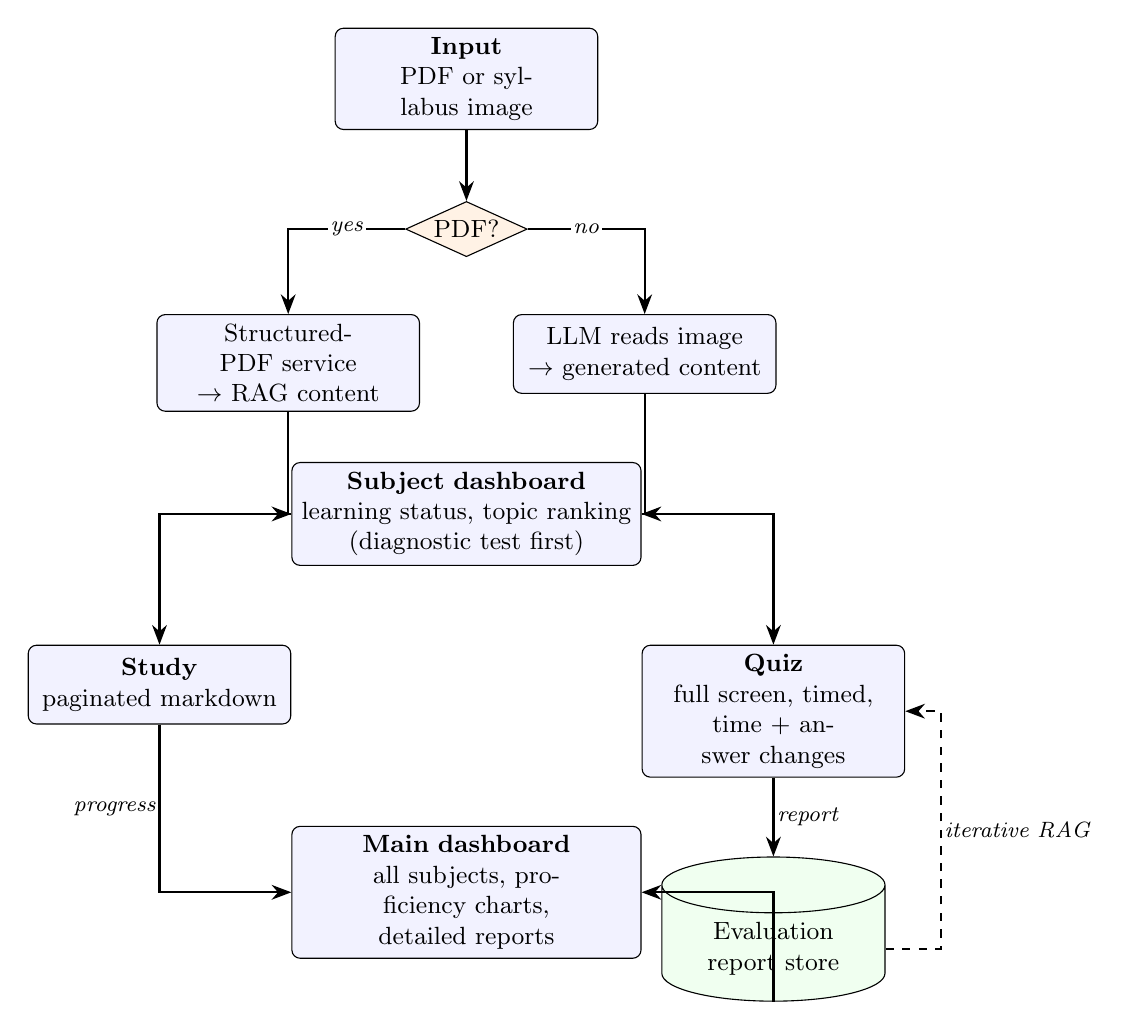
\begin{tikzpicture}[node distance=0.9cm and 0.8cm]
  \node[block] (input) {\textbf{Input}\\PDF or syllabus image};
  \node[decision, below=of input] (isPdf) {PDF?};
  \node[block, below left=0.9cm and 0.2cm of isPdf] (rag)
        {Structured-PDF service\\$\rightarrow$ RAG content};
  \node[block, below right=0.9cm and 0.2cm of isPdf] (gen)
        {LLM reads image\\$\rightarrow$ generated content};
  \node[wideblock, below=2.6cm of isPdf] (subject)
        {\textbf{Subject dashboard}\\learning status, topic ranking\\(diagnostic test first)};
  \node[block, below left=1.0cm and 0.0cm of subject] (study)
        {\textbf{Study}\\paginated markdown};
  \node[block, below right=1.0cm and 0.0cm of subject] (quiz)
        {\textbf{Quiz}\\full screen, timed,\\time + answer changes};
  \node[store, below=1.0cm of quiz] (reports) {Evaluation\\report store};
  \node[wideblock, below=3.3cm of subject] (main)
        {\textbf{Main dashboard}\\all subjects, proficiency charts,\\detailed reports};

  \draw[arr] (input) -- (isPdf);
  \draw[arr] (isPdf) -| node[lbl, pos=0.25] {yes} (rag);
  \draw[arr] (isPdf) -| node[lbl, pos=0.25] {no} (gen);
  \draw[arr] (rag) |- (subject);
  \draw[arr] (gen) |- (subject);
  \draw[arr] (subject) -| (study);
  \draw[arr] (subject) -| (quiz);
  \draw[arr] (quiz) -- node[lbl, right] {report} (reports);
  \draw[arr] (study.south) |- node[lbl, pos=0.25, left] {progress} (main.west);
  \draw[arr] (reports.south) |- (main.east);
  \draw[arr, dashed] (reports.east) -- ++(0.7,0) |- node[lbl, pos=0.25, right]
        {iterative RAG} (quiz.east);
\end{tikzpicture}
\caption{Overall architecture and learner flow of StudySense.}
\label{fig:arch}
\end{figure}

\section{Input Handling}

The platform accepts two kinds of input for a subject.

\paragraph{PDF documents.} When the learner uploads a PDF, it is sent to
the document-processing microservice described in
Section~\ref{sec:pdfservice}, which returns either the full markdown of
the document or a list of token-bounded chunks with metadata. This output
forms the retrieval corpus for the subject. Study content is then
generated topic by topic, with each generation step grounded in the
retrieved passages for that topic.

\paragraph{Syllabus images.} When the learner provides only an image of a
syllabus, there is no source text to retrieve from. The image is passed to
a vision-capable language model, which extracts the list of units and
topics and generates study content for each of them. The generated content
is stored as markdown in the same format as content derived from PDFs, so
that the rest of the system treats both cases identically.

\section{Structured-PDF Data Microservice}\label{sec:pdfservice}

PDF parsing is delegated to a separate microservice, \emph{structured-pdf-data},
which is developed in its own repository and deployed as a Docker-based
Hugging Face Space. The service is written in Python with FastAPI and uses
Docling \cite{auer2024docling} with the PyPdfium backend for conversion.
To fit the free deployment tier it runs on CPU with a single thread, and
it loads the conversion models lazily on the first request, so the first
call after a period of inactivity is slower than subsequent calls.

Chunking uses Docling's hybrid chunker with the tokenizer of the
\texttt{nvidia/llama-nemotron-embed-vl-1b-v2} embedding model, a limit of
2048 tokens per chunk and merging of small adjacent chunks under the same
heading. Each chunk is returned with a reduced set of metadata (section
headings, page numbers, element types and file name), since the complete
Docling metadata is large and of little value as LLM context.
Table~\ref{tab:endpoints} lists the endpoints of the service. All
endpoints use the HTTP GET method and take the document location in a
\texttt{source} query parameter.

\begin{table}[H]
\centering
\caption{Endpoints of the structured-pdf-data microservice.}
\label{tab:endpoints}
\begin{tabularx}{\textwidth}{@{}lX@{}}
\toprule
\textbf{Endpoint} & \textbf{Response} \\
\midrule
\texttt{/} & Health check. \\
\texttt{/get-structured-data} & Markdown of the whole document. \\
\texttt{/get-chunks-all-meta} & Chunks with the complete Docling metadata. \\
\texttt{/get-chunks} & Chunks with reduced metadata, together with the full markdown. \\
\texttt{/process-document} & Markdown if the document is small, otherwise chunks with reduced metadata. \\
\bottomrule
\end{tabularx}
\end{table}

The \texttt{/process-document} endpoint is the one used by the platform.
After conversion it measures the length of the markdown. If it is shorter
than 30{,}000 characters the markdown is returned directly, because a
document of this size can be given to the language model in a single
request without exceeding its context window, and processing it as a
whole is faster than processing chunks. Otherwise the service returns the
chunk list, so that the content can be processed in batches whose size is
chosen according to the context window of the model in use, and the
results combined afterwards. The response carries a \texttt{doc\_type}
field with the value \texttt{markdown} or \texttt{chunks} so that the
caller can tell which case applies.

\section{Study Content and Subject Dashboard}

Generated study content is stored as markdown and split into pages, each
associated with a topic. The learner reads the content one page at a time,
and the system records which pages have been studied. For each topic the
fraction of its pages not yet studied is used as a small factor in topic
ranking (Section~\ref{sec:priority}).

Each subject has its own dashboard. Before the first quiz the dashboard
shows the study material and study progress but no proficiency or
ranking, and it asks the learner to take a diagnostic test. After the
diagnostic test it shows per-topic proficiency, the knowledge-quadrant
breakdown, the topics recommended for study next, and the list of past
evaluation reports for the subject. From the subject dashboard the learner
can choose either to continue studying or to take a new evaluation.

\section{Quiz Evaluation}

The quiz is presented in full-screen mode to reduce distractions and has
an overall time limit, shown as a countdown. Questions are presented one
at a time. For each question the learner selects an answer and moves on;
there is no confidence prompt. For every question the system records the
time spent on it and the number of times the selected answer was changed.
These two quantities are the inputs to the confidence inference model of
Section~\ref{sec:inference}. When the learner finishes or the time
runs out, the responses are scored, an evaluation report is generated and
stored, and the learner is redirected to the dashboard with a confirmation
message.

\section{Scoring Model}\label{sec:scoring}

The scoring model combines a behavioural model of confidence with
certainty-based marking \cite{gardnermedwin2003} and the knowledge
quadrants of Table~\ref{tab:quadrants}. It is implemented in a single
module of the web application (\texttt{apps/web/lib/cbl.ts}).

\subsection{Inferring Confidence from Behaviour}\label{sec:inference}

StudySense does not ask the learner how sure they are. Instead, for each
answered question it uses two behavioural signals: the time $t$ (in
seconds) spent on the question and the number of times $s$ the selected
answer was changed.

\paragraph{Ideal time.} Each question is first given an ideal answering
time that accounts for the time needed to read it and to think about it:
\begin{equation}
  T_{\mathrm{ideal}} = 4 + \frac{W}{3.5} + T_{\mathrm{think}}(d),
  \label{eq:ideal}
\end{equation}
where $W$ is the number of words in the question prompt and all of its
options, $3.5$ words per second corresponds to a reading speed of about
210 words per minute, the constant $4$\,s allows for orienting to the
question and selecting an answer, and $T_{\mathrm{think}}(d)$ is a thinking
allowance that depends on the difficulty $d$ of the question:
$6$\,s for $d=1$ (recall), $12$\,s for $d=2$ (understanding, the default)
and $30$\,s for $d=3$ (calculation or multi-step reasoning).

\paragraph{Personal pace.} Learners read and work at different speeds. To
avoid interpreting a slow but secure learner as unconfident, the ideal time
is scaled by a personal pace factor
\begin{equation}
  p = \operatorname{clamp}\!\left(
      \operatorname{median}_{j \in \mathcal{C}} \frac{t_j}{T_{\mathrm{ideal},j}},
      \; 0.7,\; 1.5 \right),
  \label{eq:pace}
\end{equation}
where $\mathcal{C}$ is the set of the learner's previous \emph{correct}
answers. If fewer than five such answers are available, $p = 1$. Only
correct answers are used, so that the baseline reflects the learner's pace
when they know the material, and the clamp prevents a few extreme values
from distorting it.

\paragraph{Time ratio and time factor.} The time actually taken is
compared with the learner's personal expected time through the ratio
\begin{equation}
  r = \frac{t}{T_{\mathrm{ideal}} \cdot p},
  \label{eq:ratio}
\end{equation}
which is mapped to a time factor
\begin{equation}
  f_t =
  \begin{cases}
    0.35 & \text{if } r < 0.25, \\
    1 & \text{if } 0.25 \le r \le 1, \\
    1 - \dfrac{r - 1}{1.5} & \text{if } 1 < r < 2.5, \\
    0 & \text{if } r \ge 2.5 .
  \end{cases}
  \label{eq:timefactor}
\end{equation}
An answer given within the expected time receives full credit for
confidence. An answer given in less than a quarter of the expected time
is too fast for the question to have been read and is treated as a rushed
guess. Beyond the expected time, confidence decreases linearly and reaches
zero at two and a half times the expected time.

\paragraph{Hesitation factor.} Each change of the selected answer is taken
as a sign of hesitation:
\begin{equation}
  f_s = 0.7^{\,s}.
  \label{eq:hesitation}
\end{equation}

\paragraph{Inferred confidence and level.} The inferred confidence of an
answer is
\begin{equation}
  c = f_t \cdot f_s \in [0, 1],
  \label{eq:confidence}
\end{equation}
and it is mapped to a level: \emph{High} if $c \ge 0.7$, \emph{Medium} if
$0.4 \le c < 0.7$, and \emph{Low} if $c < 0.4$. Unanswered questions have
no confidence value; they receive zero marks and are placed in the
uninformed quadrant. Table~\ref{tab:params} lists the parameters of the
model.

\begin{table}[H]
\centering
\caption{Parameters of the confidence inference model.}
\label{tab:params}
\begin{tabularx}{\textwidth}{@{}llX@{}}
\toprule
\textbf{Symbol} & \textbf{Value} & \textbf{Meaning} \\
\midrule
--- & 4 s & Base time for orienting and selecting an answer \\
--- & 3.5 words/s & Reading speed (about 210 words per minute) \\
$W$ & per question & Words in the prompt and all options \\
$T_{\mathrm{think}}(1)$ & 6 s & Thinking allowance, recall \\
$T_{\mathrm{think}}(2)$ & 12 s & Thinking allowance, understanding (default) \\
$T_{\mathrm{think}}(3)$ & 30 s & Thinking allowance, calculation or multi-step \\
$p$ & $[0.7, 1.5]$ & Personal pace; $1$ if fewer than 5 correct answers \\
--- & $r < 0.25$ & Rushed-answer threshold, $f_t = 0.35$ \\
--- & $r \ge 2.5$ & Time at which $f_t$ reaches 0 \\
--- & 0.7 & Hesitation multiplier per answer change \\
--- & 0.7 / 0.4 & Thresholds on $c$ for High / Medium \\
\bottomrule
\end{tabularx}
\end{table}

\paragraph{Justification.} Response time (latency) is used here as an
implicit, behavioural proxy for confidence: an answer that is retrieved
readily is given promptly, while an answer the learner is unsure of tends
to come after longer deliberation or after switching between options.
Inferring confidence in this way has three practical advantages over
asking for it. It avoids self-report bias, including the miscalibration
discussed in Chapter~\ref{ch:lit}; it removes an extra click from every
question, keeping the quiz as simple as an ordinary test; and it cannot be
gamed by always claiming high confidence, since the learner never states
a confidence level.

\paragraph{Limitations.} Response time is an indirect signal. A learner may
be slow because of distraction rather than doubt, and reading speed varies
between learners; the personal pace factor mitigates the latter but not
the former. A very fast answer may also come from genuine fluency rather
than guessing, although the rushed threshold is set well below the time
needed to read the question. The constants and thresholds in
Table~\ref{tab:params} are heuristic starting values; they are to be
calibrated in the evaluation described in Section~\ref{sec:evalplan}.

\subsection{Certainty-Based Marks}

The mark for each response depends on its correctness and on its inferred
confidence level, as shown in Table~\ref{tab:cbm}. The marks are those of
certainty-based marking \cite{gardnermedwin2003}, with the level inferred
rather than chosen.

\begin{table}[H]
\centering
\caption{Certainty-based marks keyed by inferred confidence level.}
\label{tab:cbm}
\begin{tabular}{@{}lccc@{}}
\toprule
\textbf{Inferred level} & \textbf{Confidence $c$} & \textbf{Mark if correct} & \textbf{Mark if incorrect} \\
\midrule
Low    & $c < 0.4$          & $+1$ & $0$ \\
Medium & $0.4 \le c < 0.7$ & $+2$ & $-2$ \\
High   & $c \ge 0.7$        & $+3$ & $-6$ \\
\bottomrule
\end{tabular}
\end{table}

A low-confidence answer carries no risk, while an incorrect answer given
quickly and without hesitation is penalised heavily, because it indicates
a firmly held misconception.

\subsection{Quadrant Classification}

A response is considered \emph{confident} if its inferred level is High or
Medium, and \emph{not confident} if it is Low. Each response is then
classified as shown in Table~\ref{tab:classify}.

\begin{table}[H]
\centering
\caption{Classification of a response into a knowledge quadrant.}
\label{tab:classify}
\begin{tabularx}{\textwidth}{@{}llX@{}}
\toprule
\textbf{Correct?} & \textbf{Inferred level} & \textbf{Quadrant and interpretation} \\
\midrule
Yes & High or Medium & Mastery \\
Yes & Low            & Doubt: correct but slow or hesitant \\
No  & High or Medium & Misinformed: answered quickly and wrongly, a misconception \\
No  & Low            & Uninformed: wrong and hesitant \\
No  & (unanswered)   & Uninformed, zero marks \\
\bottomrule
\end{tabularx}
\end{table}

\subsection{Topic Proficiency}

Every question belongs to a topic. For a topic $t$ with $n_t$ questions in
a quiz and marks $m_1, \dots, m_{n_t}$, the proficiency is
\begin{equation}
  P_t = \frac{\max\!\left(0, \sum_{i=1}^{n_t} m_i\right)}{3\,n_t} \times 100 .
  \label{eq:proficiency}
\end{equation}
The denominator $3\,n_t$ is the highest possible mark for the topic, so
$P_t$ lies between $0$ and $100$; a topic reaches $100$ only if every
question was answered correctly with High inferred confidence. Negative
totals, which arise from confident errors, are clipped to zero.

\subsection{Topic Priority for the Next Quiz}\label{sec:priority}

For each topic the system computes a priority that determines how strongly
the topic is targeted in the next quiz:
\begin{equation}
  \mathrm{priority}_t = \left(1 - \frac{P_t}{100}\right)
    + 0.5 \times s^{\mathrm{mis}}_t
    + 0.1 \times u_t ,
  \label{eq:priority}
\end{equation}
where $s^{\mathrm{mis}}_t$ is the share of the topic's responses that fell
in the misinformed quadrant and $u_t$ is the fraction of the topic's study
pages that the learner has not yet studied. The first term favours topics
with low proficiency, the second gives extra weight to confident errors in
line with the hypercorrection effect \cite{butterfield2001}, and the third
adds a small factor for material the learner has not yet read.

\subsection{Recorded Quantities}

For every response the report records the question, the selected and
correct answers, the time taken, the ideal time, the number of answer
changes, the inferred confidence value and level, the mark, the quadrant, the topic
and the time taken in seconds. For the quiz as a whole it records the
total mark, the accuracy, the per-topic proficiency, the quadrant counts
and the total time. The learner's personal pace is updated from the
correct answers of each completed quiz.

\section{Iterative Retrieval-Augmented Generation}

Every evaluation report is stored in full. Whenever a new quiz is
generated for a subject, all previous evaluation reports for that subject
are supplied to the generator together with the relevant study content.
The generator is instructed to select topics and questions in the
following order:
\begin{enumerate}
  \item topics with responses in the \textbf{misinformed} quadrant, so that
        confident errors are confronted and corrected;
  \item topics in the \textbf{uninformed} quadrant, to close known gaps;
  \item topics in the \textbf{doubt} quadrant, to consolidate fragile
        knowledge \cite{butler2008};
  \item occasional re-tests of \textbf{mastery} topics, to check retention
        over time \cite{ebbinghaus1885}.
\end{enumerate}
Within these groups, topics are ordered by the priority of
Equation~\eqref{eq:priority}. Because each new quiz produces a new report,
the retrieval context grows with every iteration and the generated quizzes
follow the learner's changing knowledge state. The loop corresponds to the
diagnose--prescribe--learn--iterate cycle of confidence-based learning,
continued until all topics reach mastery.

\begin{figure}[H]
\centering
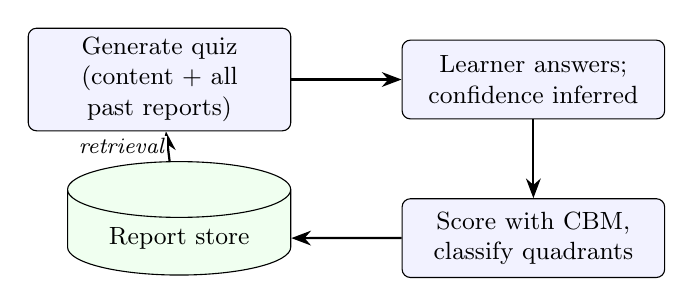
\begin{tikzpicture}[node distance=1.0cm and 1.4cm]
  \node[block] (gen) {Generate quiz\\(content + all past reports)};
  \node[block, right=of gen] (take) {Learner answers;\\confidence inferred};
  \node[block, below=of take] (score) {Score with CBM,\\classify quadrants};
  \node[store, left=of score] (store) {Report store};
  \draw[arr] (gen) -- (take);
  \draw[arr] (take) -- (score);
  \draw[arr] (score) -- (store);
  \draw[arr] (store) -- node[lbl, left] {retrieval} (gen);
\end{tikzpicture}
\caption{The iterative retrieval-augmented generation loop over evaluation reports.}
\label{fig:loop}
\end{figure}

\section{Dashboards and Reports}

The main dashboard lists all subjects the learner has added, with the
proficiency of each subject and charts of proficiency across successive
evaluations. For each subject it shows the study reports and the topics
covered so far, together with all evaluation reports. Each evaluation
report summarises which topics are strong and which are weak and which
answers were correct or incorrect; selecting a report opens a detailed
view showing every question, the learner's answer, the correct answer,
the inferred confidence value, the mark, the quadrant and the time taken.
The report screen also shows a chart comparing, for each question, the
time taken with the ideal time, which makes rushed and hesitant answers
easy to see.

% --------------------------------------------------------------------------
\chapter{Implementation}\label{ch:impl}
% --------------------------------------------------------------------------

\section{Repository Structure}

The platform is organised as a monorepo managed with Turborepo
\cite{turborepo} and npm workspaces. A monorepo keeps the web application,
the API and the shared packages in a single repository with a single
dependency installation, while Turborepo runs build and type-check tasks
across the packages in dependency order. The layout is shown in
Figure~\ref{fig:repo}.

\begin{figure}[H]
\centering
\begin{minipage}{0.85\textwidth}
\small
\begin{verbatim}
minor/
|-- apps/
|   |-- web/             Next.js web application (port 3000)
|   `-- api/             Express API (port 4000)
|-- packages/
|   |-- pdf-client/      typed client for structured-pdf-data
|   `-- config/          shared TypeScript configuration
|-- context/             project design notes and decisions
|-- utils/               project report and presentation
|-- package.json         workspaces and root scripts
`-- turbo.json           task pipeline
\end{verbatim}
\end{minipage}
\caption{Repository layout of the monorepo.}
\label{fig:repo}
\end{figure}

The document-processing microservice is kept in a separate repository and
deployed independently, because it has a different language, runtime and
resource profile from the rest of the system. The monorepo communicates
with it only over HTTP, through the address configured in the
\texttt{PDF\_SERVICE\_URL} environment variable.

\section{Web Application}

The web application in \texttt{apps/web} is built with Next.js
\cite{nextjs} version 16 using the App Router and TypeScript. It
contains the screens described in Chapter~\ref{ch:method}: subject
creation from a PDF or syllabus image, the main dashboard, the subject
dashboard, the paginated study reader, the full-screen timed quiz, which
records time and answer changes for each question, and the detailed
evaluation report with its time-versus-ideal-time chart. The confidence
inference and scoring model of Section~\ref{sec:scoring} is implemented in
a single module (\texttt{lib/cbl.ts}) so that the same rules are applied wherever reports are computed or
displayed. In the current phase all data access goes through one data
module backed by mock data, so that it can later be replaced by calls to
the API without changes to the screens.

\section{API Server}

The API in \texttt{apps/api} is built with Express \cite{express} version 5
and TypeScript, executed with \texttt{tsx}. In the current phase it
exposes a health endpoint and two endpoints that forward requests to the
document-processing microservice: one that reports the health of the
service and one that processes a document given its URL. The API is the
only component that calls the microservice; the browser communicates only
with the API. In the next phase the API will also host content and quiz
generation, the iterative RAG loop and persistence.

\section{Shared PDF Client}

The package \texttt{@minor/pdf-client} provides a typed client for the
microservice. It defines TypeScript types for chunks and for the two
possible responses of \texttt{/process-document}, and it exposes functions
for the health check, for retrieving the markdown of a document, for
retrieving chunks, and for the combined processing endpoint. The base
address of the service is configurable and defaults to the deployed Hugging
Face Space. Because the package exports its TypeScript source directly, it
does not require a separate build step.

\section{Planned Persistence and Language Model Integration}

Persistent storage is planned on PostgreSQL accessed through the Prisma
ORM \cite{prisma}. The main entities are subjects, topics, study pages and
study progress, quizzes, responses and evaluation reports. The pgvector
extension will store embeddings of document chunks in the same database,
so that retrieval for content and quiz generation can be performed with a
vector similarity query without a separate vector store.

The choice of language model provider has been deliberately left open.
Generation will be accessed through a small provider-independent
interface, so that the provider can be selected later on the basis of
cost, support for image input (needed for syllabus images) and context
window size (needed to supply all previous evaluation reports).

\section{Technology Stack}

Table~\ref{tab:stack} summarises the technologies used and planned.

\begin{table}[H]
\centering
\caption{Technology stack of the platform.}
\label{tab:stack}
\begin{tabularx}{\textwidth}{@{}llX@{}}
\toprule
\textbf{Layer} & \textbf{Technology} & \textbf{Role} \\
\midrule
Monorepo        & Turborepo, npm workspaces & Task pipeline and shared dependencies \\
Web application & Next.js 16, React, TypeScript & User interface, quiz and dashboards \\
API             & Express 5, TypeScript, tsx & Orchestration and service access \\
Shared client   & \texttt{@minor/pdf-client} & Typed access to the PDF service \\
PDF service     & Python, FastAPI \cite{fastapi}, Docling & PDF to markdown and chunks \\
Deployment      & Docker, Hugging Face Spaces & Hosting of the PDF service \\
Database (planned) & PostgreSQL, Prisma, pgvector & Persistence and vector retrieval \\
Language model (planned) & Provider-independent interface & Content, quiz and report generation \\
\bottomrule
\end{tabularx}
\end{table}

\section{Current Status}

At the time of writing the following components are complete:
\begin{itemize}
  \item the monorepo structure, build pipeline and shared configuration;
  \item the structured-pdf-data microservice, deployed and reachable;
  \item the typed PDF client and the API endpoints that use it, verified
        against the deployed service;
  \item the web interface for all screens of Chapter~\ref{ch:method}, operating on
        mock data, including the confidence inference and scoring model.
\end{itemize}
The following components are planned for the next phase:
\begin{itemize}
  \item persistent storage with PostgreSQL, Prisma and pgvector;
  \item integration of a language model for content, quiz and report
        generation, including syllabus images;
  \item the iterative RAG loop operating on stored reports;
  \item connection of the web interface to the API.
\end{itemize}

\section{Evaluation Plan}\label{sec:evalplan}

No learner study has been carried out yet, and this report makes no claim
about learning outcomes. The planned evaluation has three parts.

\paragraph{Functional evaluation.} Each stage of the pipeline will be
tested end to end with a set of PDFs of different sizes and structures and
with syllabus images of different quality. For PDF input, the extracted
markdown and chunks will be checked for preserved headings and tables, and
both branches of the 30,000-character rule will be exercised.

\paragraph{Quality of generated content and questions.} A sample of
generated study pages and quiz questions will be reviewed manually for
factual correctness against the source material, relevance to the
assigned topic and clarity of the answer options. Questions generated with
and without past reports in the context will be compared to check that the
iterative RAG loop does shift questions towards weak topics.

\paragraph{Calibration of the confidence model.} Because the constants
and thresholds of the inference model are heuristic, a pilot will be run
in which learners answer quizzes normally and, after each answer, also
report their confidence on a three-level scale. The inferred levels will be
compared with the self-reported levels, and the agreement between them
will be measured. The ideal-time constants, the rushed threshold, the
hesitation multiplier and the level thresholds will then be adjusted to
improve agreement, and the correctness rate within each inferred level
will be checked to confirm that higher inferred confidence corresponds to
a higher probability of being correct. The self-report prompt is used only
in this pilot, not in the product.

\paragraph{Effect on learning.} A small study with student volunteers is
planned in which one group uses the full confidence-based loop and a
second group uses the same content with conventional correctness-only
quizzes. Outcomes to be compared include accuracy on a final test, the
proportion of responses in the misinformed quadrant over successive
quizzes, calibration of the inferred confidence (agreement between
inferred confidence and actual correctness), and the number of quizzes needed for topics to
reach mastery. Results will be reported only after the study is carried
out.

% --------------------------------------------------------------------------
\chapter{Conclusion and Future Work}\label{ch:concl}
% --------------------------------------------------------------------------

\section{Conclusion}

This report has presented the design and prototype implementation of an
adaptive study platform, StudySense, built on confidence-based learning.
Instead of recording only whether an answer is correct, StudySense infers
the learner's confidence in every answer from behaviour, namely the time
taken relative to a question-specific ideal time scaled by the learner's
personal pace, and the number of answer changes, without asking the
learner to rate it. It then scores responses with certainty-based marking, and classifies them into the four knowledge
quadrants of mastery, doubt, misinformation and uninformed. This makes it
possible to identify the learners and topics that conventional scoring
misses: correct answers that are only guesses or held with doubt, and
incorrect answers that the learner believes to be right.

StudySense turns these results into action through an iterative
retrieval-augmented generation loop. Study content is generated from the
learner's own PDF material, processed by a Docling-based microservice, or
from an image of the syllabus, and every evaluation report is stored and
supplied to the generation of the next quiz. New quizzes therefore
prioritise misinformed topics, then knowledge gaps, then fragile
knowledge, and periodically re-test mastered topics, following the
diagnose--prescribe--learn--iterate cycle until mastery is reached.

The system is organised as a Turborepo monorepo with a Next.js web
application, an Express API and a shared typed client for the
independently deployed document-processing service. The current phase
delivers the full user interface on mock data, the scoring model and a
working integration with the document service.

\section{Future Work}

The immediate next steps are to implement persistent storage on
PostgreSQL with Prisma and pgvector, to integrate a language model for
content, quiz and report generation, and to connect the web interface to
the API so that the iterative RAG loop operates on real stored reports.
Once the full loop is in place, the evaluation plan of the previous
chapter will be carried out, beginning with the calibration of the
confidence inference model against self-reported confidence, and then
measuring the effect of the confidence-based approach on learning
outcomes.

Further extensions include spaced scheduling of mastery re-tests based on
the time since a topic was last tested, additional behavioural signals
for confidence inference such as focus loss during a question, question formats beyond multiple
choice, and support for groups of learners so that an instructor can see
the knowledge-quadrant profile of a whole class.

% ==========================================================================
%  BIBLIOGRAPHY
% ==========================================================================
\begin{thebibliography}{99}
\addcontentsline{toc}{chapter}{Bibliography}

\bibitem{benchprep}
BenchPrep, ``Why confidence-based learning improves performance,''
BenchPrep Blog. [Online]. Available:
\url{https://blog.benchprep.com/why-confidence-based-learning-improves-performance}
(accessed Nov. 2026).

\bibitem{gardnermedwin2003}
A. R. Gardner-Medwin and M. Gahan, ``Formative and summative
confidence-based assessment,'' in \emph{Proc. 7th Int. Computer-Aided
Assessment Conf.}, Loughborough, U.K., 2003.

\bibitem{butterfield2001}
B. Butterfield and J. Metcalfe, ``Errors committed with high confidence are
hypercorrected,'' \emph{Journal of Experimental Psychology: Learning,
Memory, and Cognition}, vol. 27, no. 6, pp. 1491--1494, 2001.

\bibitem{butler2008}
A. C. Butler, J. D. Karpicke, and H. L. Roediger III, ``Correcting a
metacognitive error: Feedback increases retention of low-confidence
correct responses,'' \emph{Journal of Experimental Psychology: Learning,
Memory, and Cognition}, vol. 34, no. 4, pp. 918--928, 2008.

\bibitem{roediger2006}
H. L. Roediger III and J. D. Karpicke, ``Test-enhanced learning: Taking
memory tests improves long-term retention,'' \emph{Psychological Science},
vol. 17, no. 3, pp. 249--255, 2006.

\bibitem{kruger1999unskilled}
J. Kruger and D. Dunning, ``Unskilled and unaware of it: How difficulties in
recognizing one's own incompetence lead to inflated self-assessments,''
\emph{Journal of Personality and Social Psychology}, vol. 77, no. 6,
pp. 1121--1134, 1999.

\bibitem{bloom1984}
B. S. Bloom, ``The 2 sigma problem: The search for methods of group
instruction as effective as one-to-one tutoring,'' \emph{Educational
Researcher}, vol. 13, no. 6, pp. 4--16, 1984.

\bibitem{ebbinghaus1885}
H. Ebbinghaus, \emph{\"Uber das Ged\"achtnis: Untersuchungen zur
experimentellen Psychologie}. Leipzig, Germany: Duncker \& Humblot, 1885.

\bibitem{lewis2020rag}
P. Lewis \emph{et al.}, ``Retrieval-augmented generation for
knowledge-intensive NLP tasks,'' in \emph{Advances in Neural Information
Processing Systems (NeurIPS)}, vol. 33, 2020.

\bibitem{auer2024docling}
C. Auer \emph{et al.}, ``Docling technical report,'' arXiv preprint
arXiv:2408.09869, 2024.

\bibitem{turborepo}
Vercel, ``Turborepo documentation.'' [Online]. Available:
\url{https://turborepo.com/docs} (accessed Nov. 2026).

\bibitem{nextjs}
Vercel, ``Next.js documentation.'' [Online]. Available:
\url{https://nextjs.org/docs} (accessed Nov. 2026).

\bibitem{express}
OpenJS Foundation, ``Express documentation.'' [Online]. Available:
\url{https://expressjs.com} (accessed Nov. 2026).

\bibitem{fastapi}
S. Ram\'irez, ``FastAPI documentation.'' [Online]. Available:
\url{https://fastapi.tiangolo.com} (accessed Nov. 2026).

\bibitem{prisma}
Prisma, ``Prisma ORM documentation.'' [Online]. Available:
\url{https://www.prisma.io/docs} (accessed Nov. 2026).

\end{thebibliography}

\end{document}
